\documentclass[../main.tex]{subfiles}
En este capítulo se recogen las pruebas realizadas a la estación de tierra. A partir de los resultados obtenidos tanto en simulación como en pruebas reales se persigue su validación experimental. Estos experimentos han de comprobar que los objetivos planteados en este proyecto se cumplen. \\
Además de las pruebas unitarias de diferentes partes de la aplicación realizadas para verificar los casos de uso, en este capítulo se detallan las pruebas integrales de vuelo realizadas. Estas pruebas se han realizado tanto en simulación como en con la aeronave real. \\
Principalmente, se han realizado dos pruebas de vuelo. Ambos experimentos en simulación y con una aeronave real de ala rotatoria, el 3DR Solo Drone (ver Figura \ref{fig:3dr}). En uno se ha realizado con una misión polilínea mientras que el otro con una misión por patrón. Estos test de vuelo de la aplicación se verán con profundidad en las secciones de este capítulo. \\
También se adjunta una lista de reproducción \footnote{https://www.youtube.com/playlist?list=PLGlX46StCA-QAXmeQp5omNhllGJ3CMjcO} que recoge la evolución de la aplicación a lo largo del tiempo con las distintas versiones realizadas. Aproximadamente cada mes se ha grabado un vídeo con las principales novedades de desarrollo durante ese periodo. Esta lista muestra una visión de las características de la aplicación y de los tiempos de desarrollo empleados. \\
Para realizar las pruebas de vuelo en real ha sido necesario desplazarse a un campo de vuelo donde se cumpliese la legislación actual. En campo de vuelo elegido ha sido el de Seseña \cite{campo-vuelo}. La Figura \ref{fig:campo-vuelo} muestra parte de las instalaciones y el despliegue realizado durante las pruebas.

\begin{figure}[h]
    \centering
    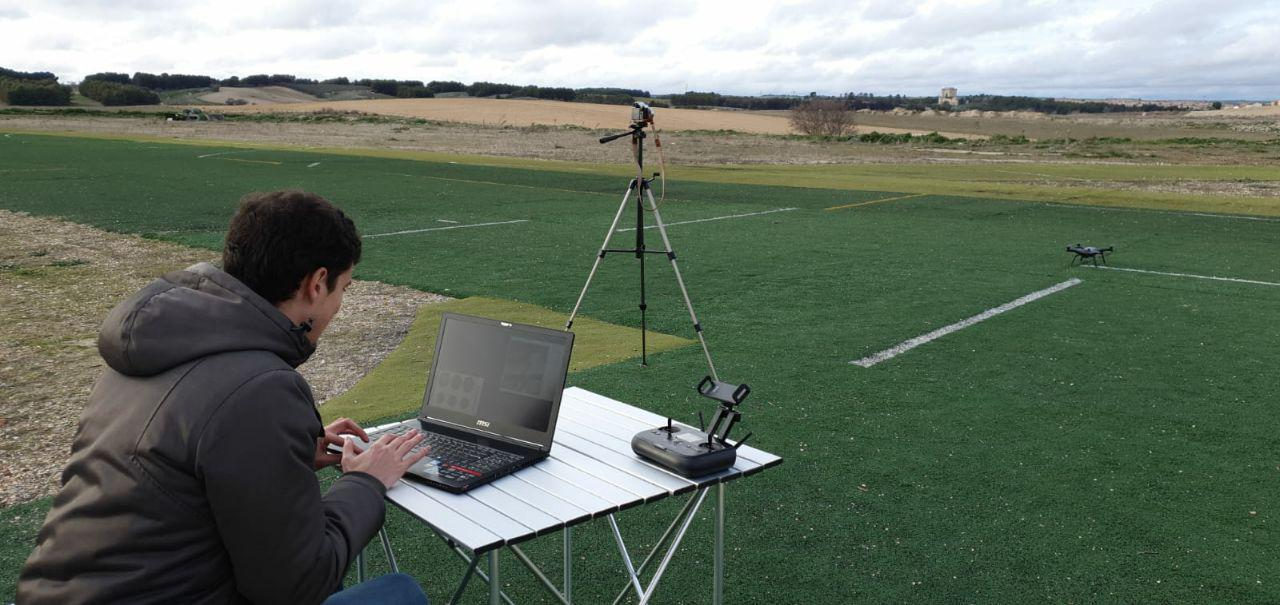
\includegraphics[width=0.9\textwidth]{prueba-vuelo.jpg}
    \caption{Campo de vuelo de Seseña.}
    \label{fig:campo-vuelo}
\end{figure}

\section{Misión polilínea en simulación.}
Este experimento realiza en un entorno de simulación la creación de una misión polilínea, el envío a la aeronave y el seguimiento de la misión. La simulación permite la detección de errores sin poner en riesgo a la aeronave. La Figura \ref{fig:sim-pol} contiene unas capturas de pantalla realizadas durante la simulación. La secuencia de ejecución seguida ha sido:

\begin{enumerate}
    \item Lanzamiento de la simulación mediante un SITL de PX4 con Gazebo9. Ejecución de la aplicación.
    \item Establecimiento de la conexión entre estación terrestre y aeronave (ver caso de uso \ref{subsection:results-caso4}).
    \item Caracterización de la aeronave y carga de pago (ver caso de uso \ref{subsection:results-caso1}). Este paso, pese haberlo realizado, resulta prescindible para las misiones polilínea.
    \item Creación de la misión polilínea (ver caso de uso \ref{subsection:results-caso3} y Fig. \ref{fig:sim-pol1}).
    \item Validación de la misión creada.
    \item Comprobaciones pre-vuelo y envío de la misión a la aeronave.
    \item Inicio de la misión y seguimiento de la misma (ver caso de uso \ref{subsection:results-caso6} y Fig. \ref{fig:sim-pol2}).
    \item Aterrizaje y fin de la misión.
\end{enumerate}

\begin{figure}[h]
    \begin{subfigure}{0.5\textwidth}
        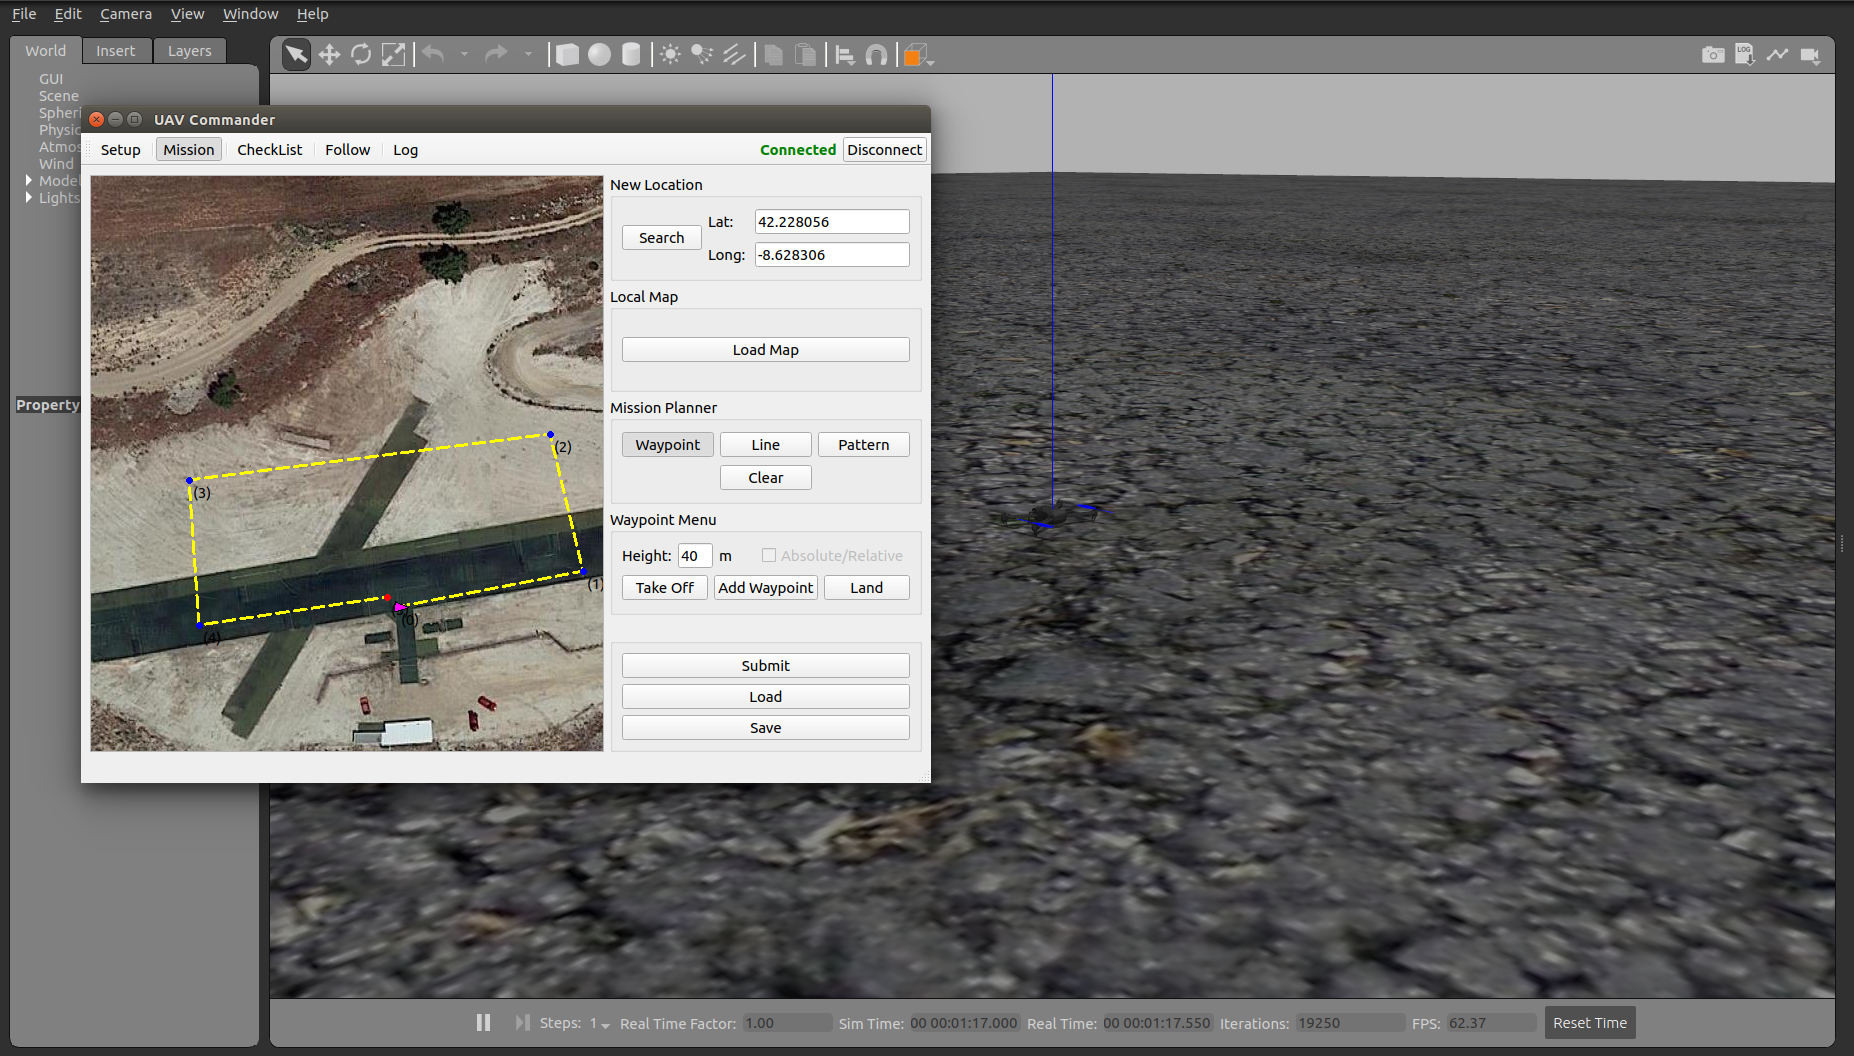
\includegraphics[width=0.9\linewidth]{sim-pol-1.png}
        \caption{Simulación de la creación de la misión.}
        \label{fig:sim-pol1}
    \end{subfigure}
    \begin{subfigure}{0.5\textwidth}
        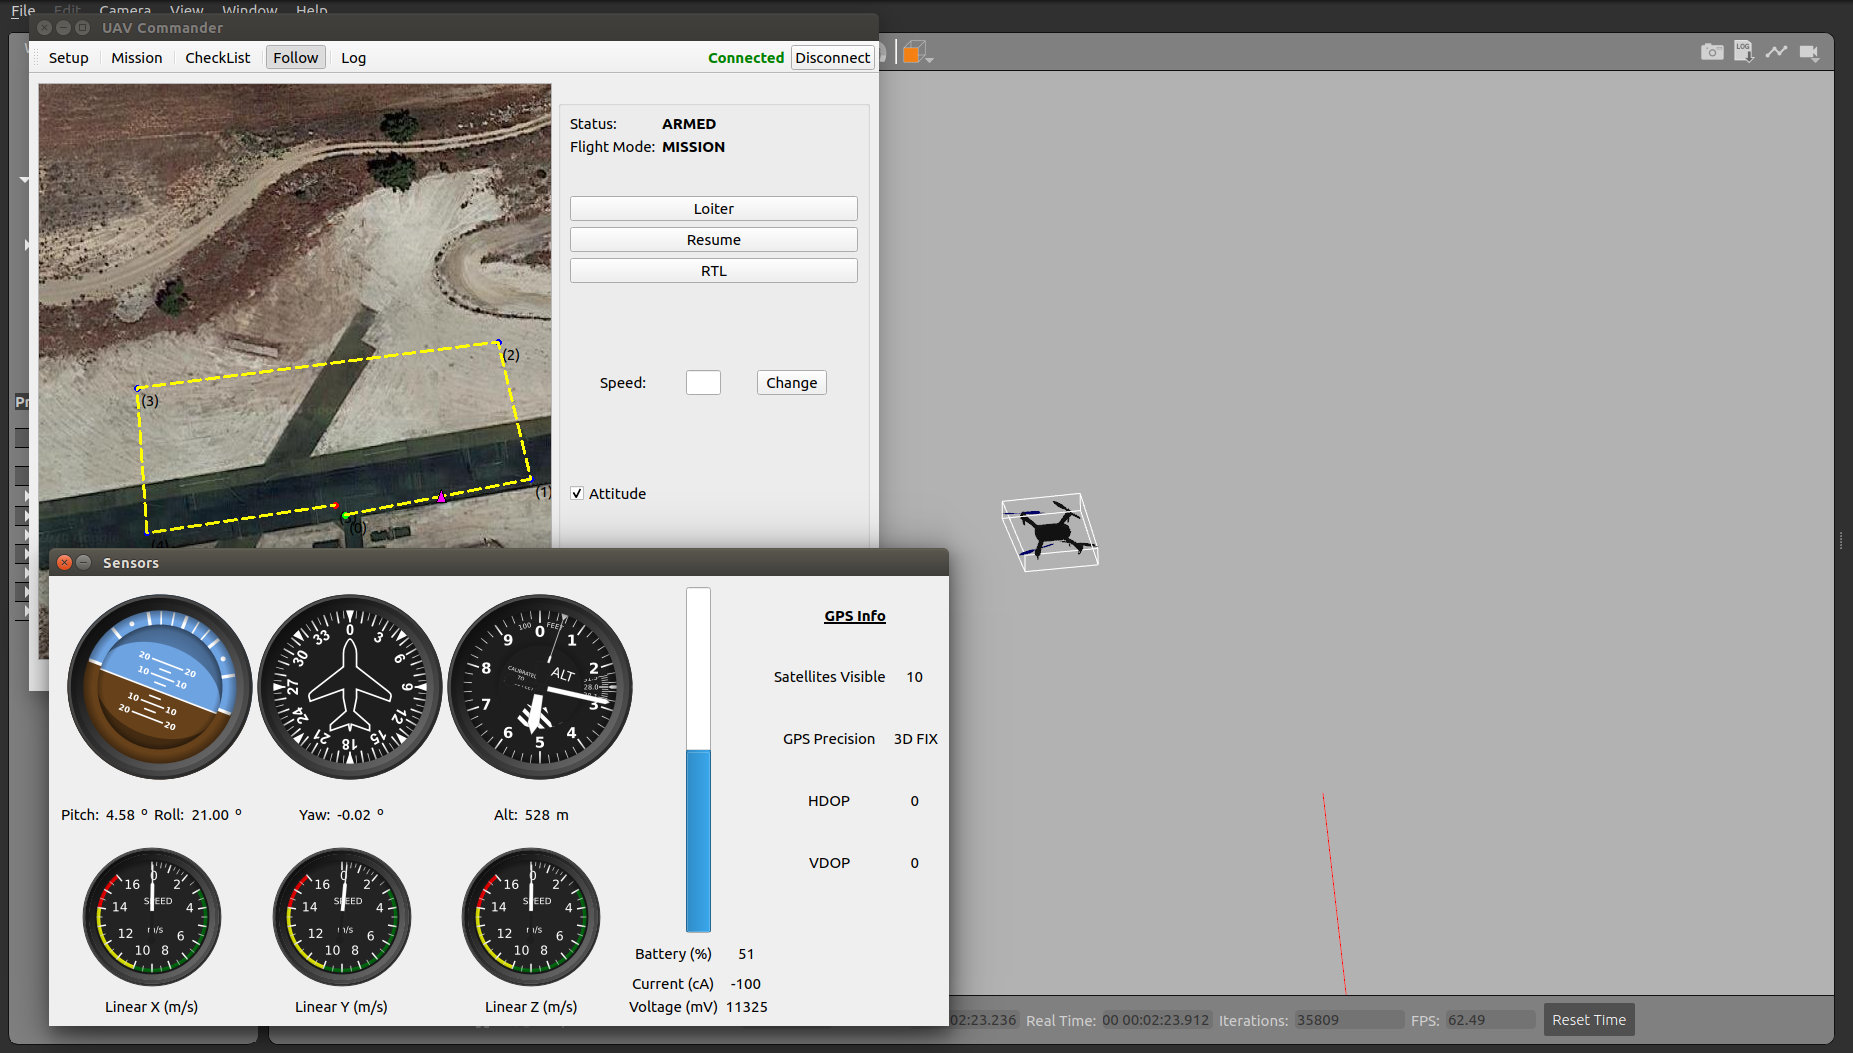
\includegraphics[width=0.9\linewidth]{sim-pol-2.png}
        \caption{Simulación del seguimiento de la misión.}
        \label{fig:sim-pol2}
    \end{subfigure}

    \caption{Simulación de vuelo para misiones polilínea.}
    \label{fig:sim-pol}
\end{figure}

Tras realizar la prueba en simulación y comprobar el buen funcionamiento de la aplicación se considera que el software ya está listo para realizar pruebas en real. Esta prueba en real se muestra en la siguiente sección.

\section{Prueba de vuelo real para misiones polilínea.}
Este experimento reproduce un supuesto en el cual un operario realiza una misión polilínea \emph{in situ}, la envía a la aeronave y realiza el seguimiento de la misma. Para documentar la prueba de vuelo se ha generado un vídeo del que se adjunta su enlace \footnote{https://youtu.be/UOv8Go\_Q22k}. La Figura \ref{fig:prueba-pol} muestra una serie de fotogramas del vídeo mencionado. \\

La secuencia de ejecución seguida durante el experimento ha sido la siguiente:

\begin{enumerate}
    \item Ejecución de la aplicación y encendido del 3DR Solo junto a su emisora.
    \item Establecimiento de conexión entre ambos cuando el 3DR Solo ha establecido señal GPS (ver caso de uso \ref{subsection:results-caso4}).
    \item Caracterización de la aeronave y carga de pago (ver caso de uso \ref{subsection:results-caso1}). Este paso, pese haberlo realizado, resulta prescindible para las misiones polilínea.
    \item Creación de la misión polilínea (ver caso de uso \ref{subsection:results-caso3} y  Fig. \ref{fig:prueba-pol1}).
    \item Validación de la misión creada.
    \item Comprobaciones pre-vuelo y envío de la misión a la aeronave (Fig. \ref{fig:prueba-pol2}).
    \item Inicio de la misión y seguimiento de la misma (ver caso de uso \ref{subsection:results-caso6} y Fig. \ref{fig:prueba-pol3}).
    \item Aterrizaje y fin de la misión (Fig. \ref{fig:prueba-pol4}).
\end{enumerate}

% Es importante destacar que desde el momento de grabación del vídeo la aplicación ha seguido evolucionando y su versión actual es ligeramente diferente al momento del ensayo. Las diferencias son aspectos menores, pues las funcionalidades son prácticamente las mismas.

% \begin{figure}[h]
%    \centering
%    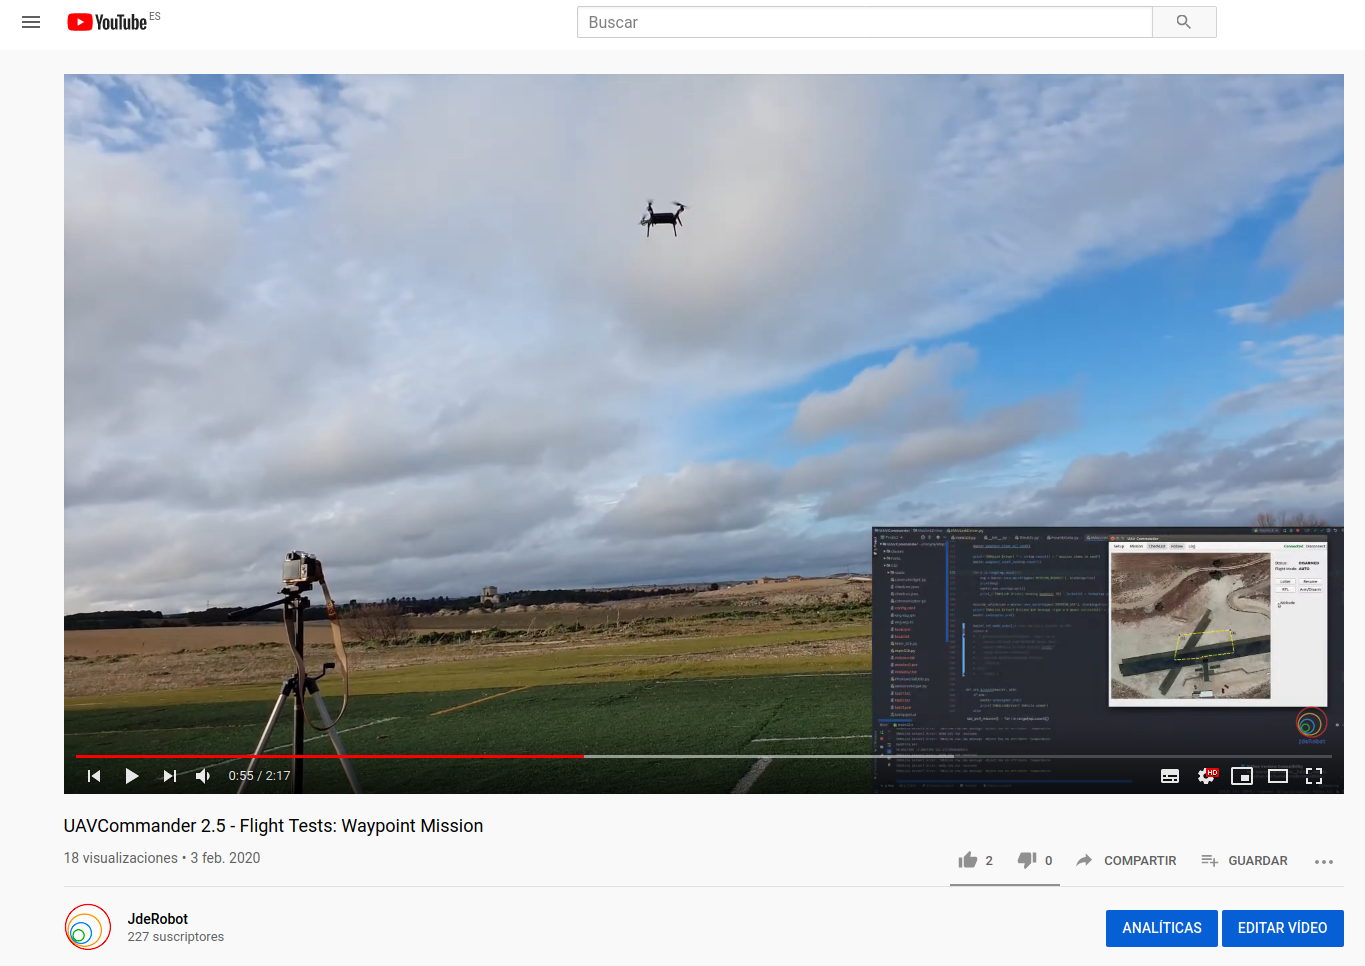
\includegraphics[width=0.9\textwidth]{prueba-pol.png}
%    \caption{Vídeo con la prueba de vuelo para misiones polilínea.}
%    \label{fig:prueba-pol}
% \end{figure}

\begin{figure}[h]
    \begin{subfigure}{0.5\textwidth}
        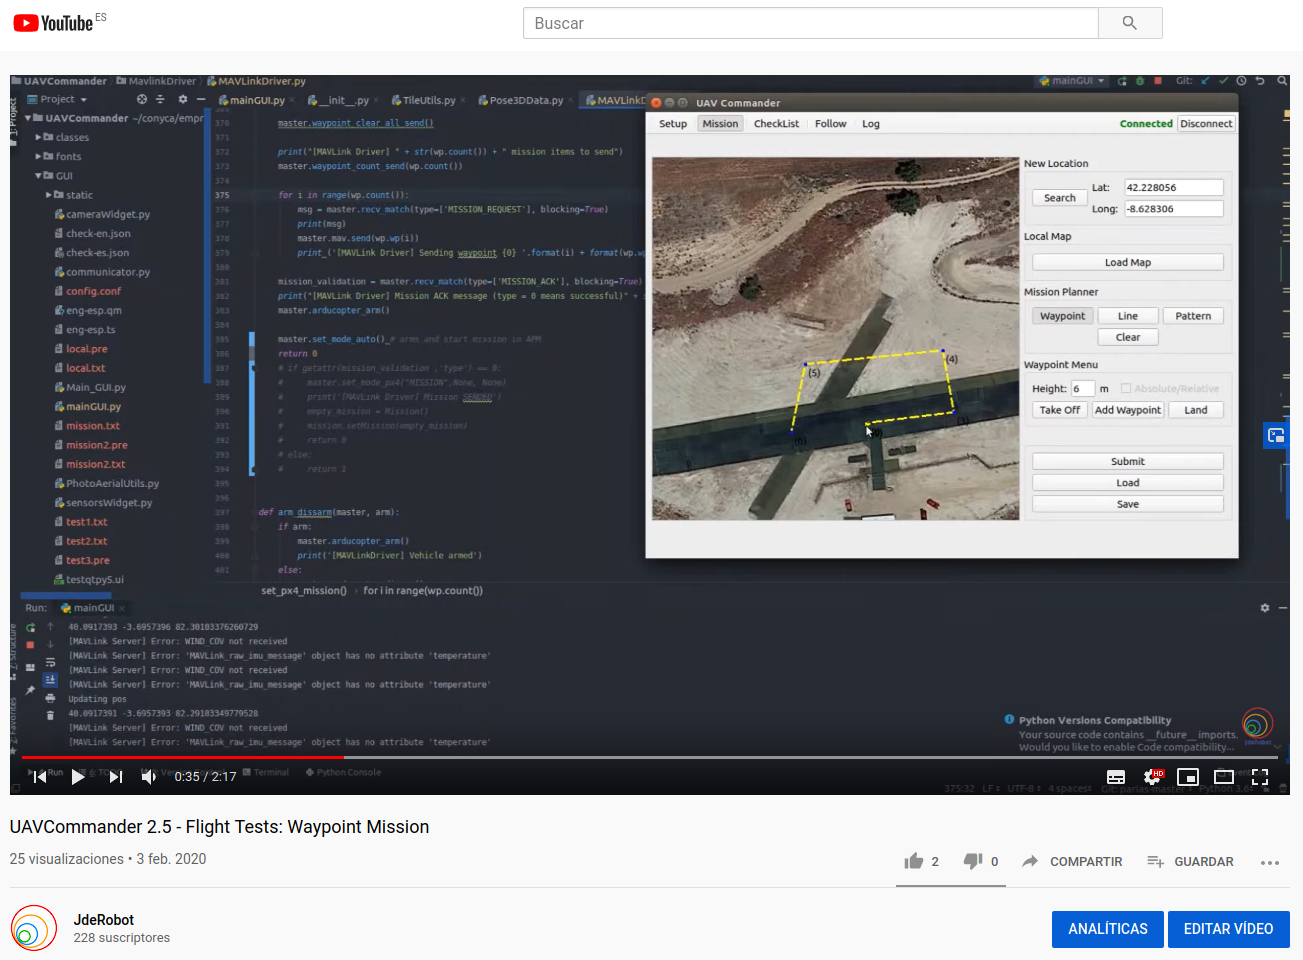
\includegraphics[height=6cm, width=0.9\linewidth]{prueba-pol-1.png}
        \caption{Creación de la misión polilínea.}
        \label{fig:prueba-pol1}
    \end{subfigure}
    \begin{subfigure}{0.5\textwidth}
        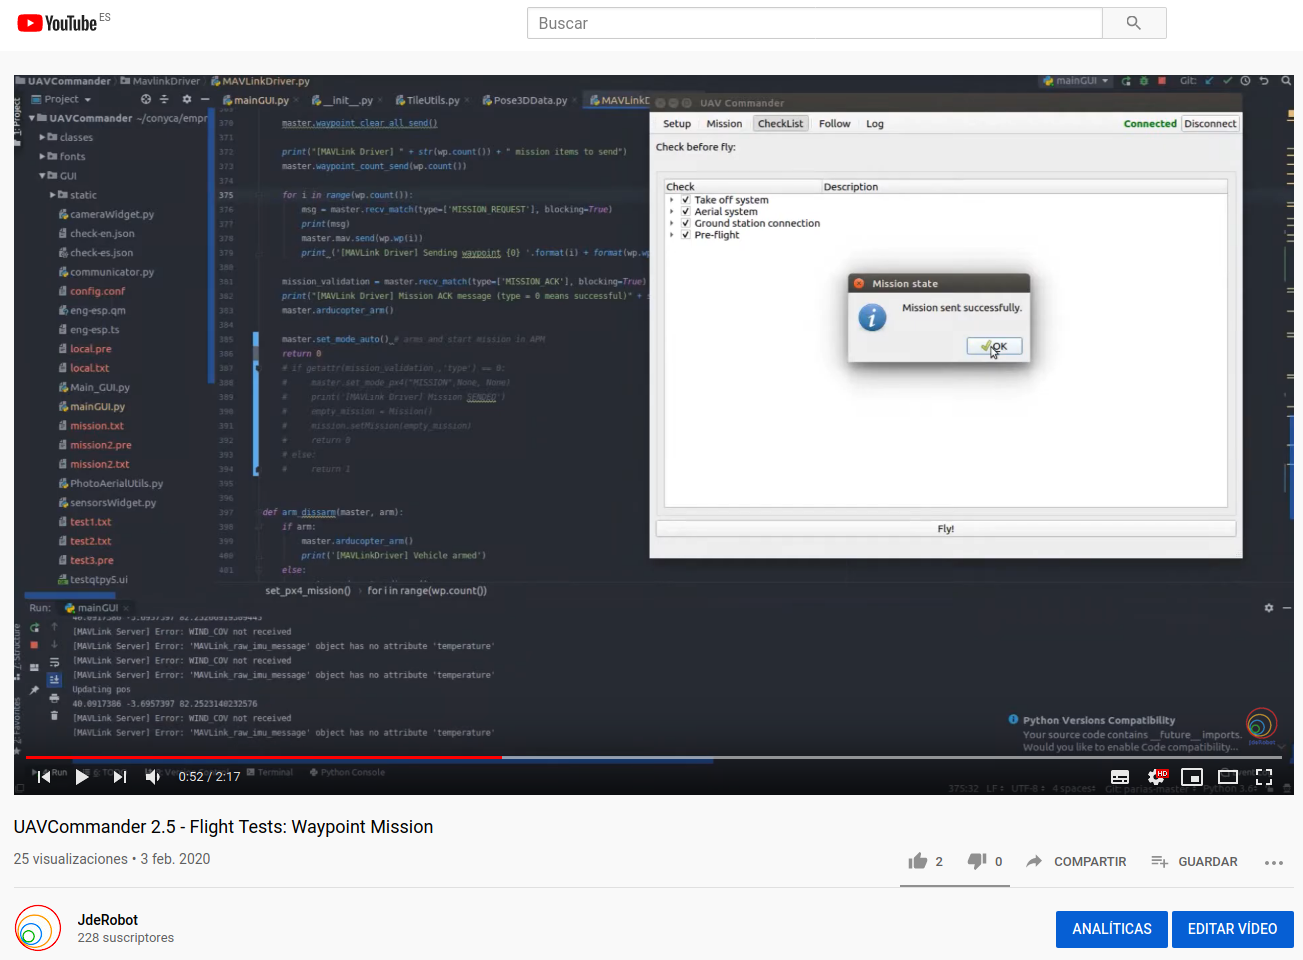
\includegraphics[height=6cm, width=0.9\linewidth]{prueba-pol-2.png}
        \caption{Envío de misión a aeronave.}
        \label{fig:prueba-pol2}
    \end{subfigure}
        
    \begin{subfigure}{0.5\textwidth}
        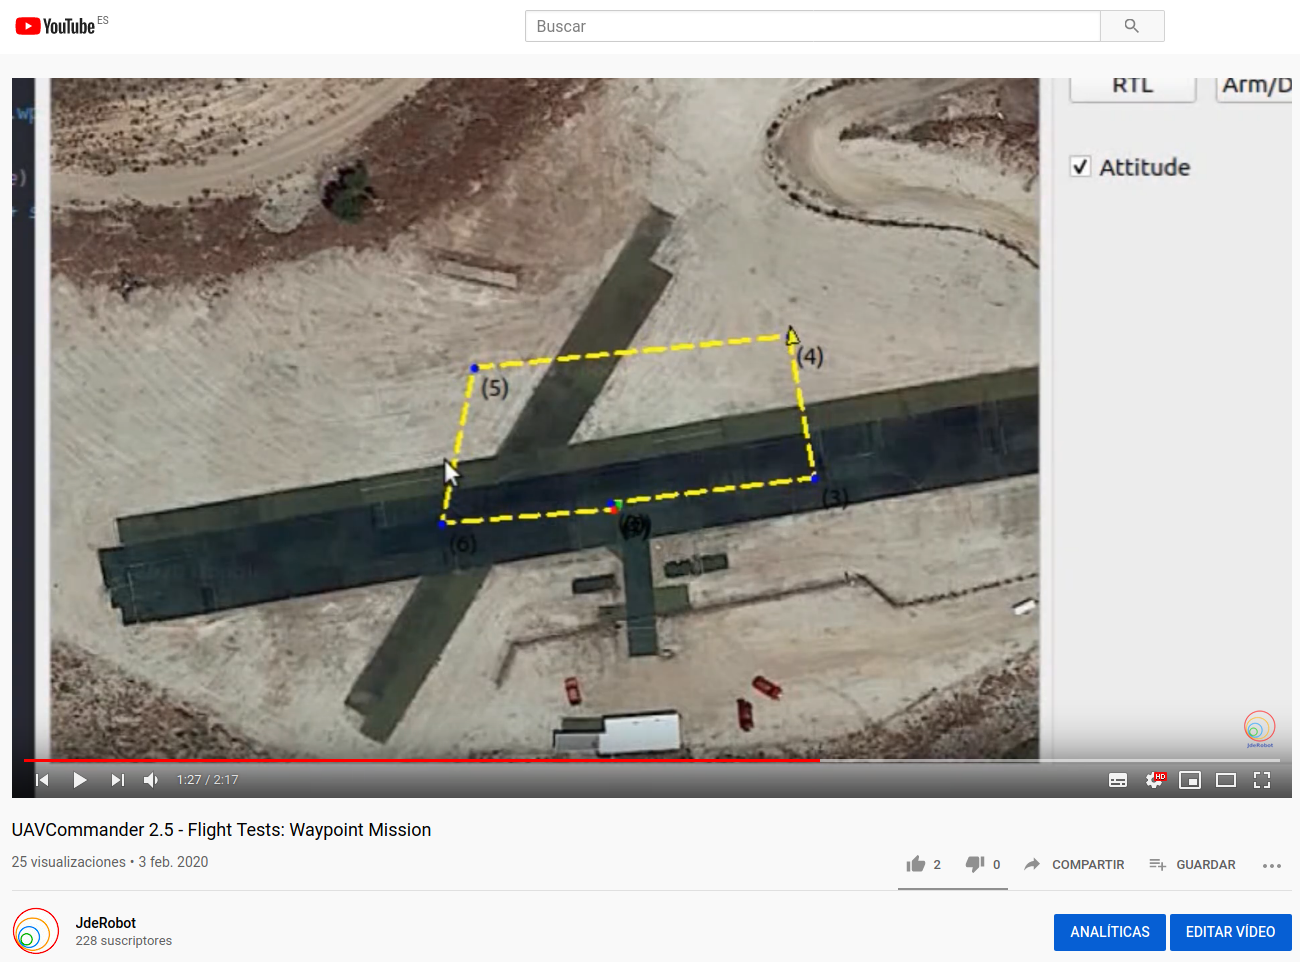
\includegraphics[height=6cm, width=0.9\linewidth]{prueba-pol-3.png}
        \caption{Seguimiento de la misión.}
        \label{fig:prueba-pol3}
    \end{subfigure}
    \begin{subfigure}{0.5\textwidth}
        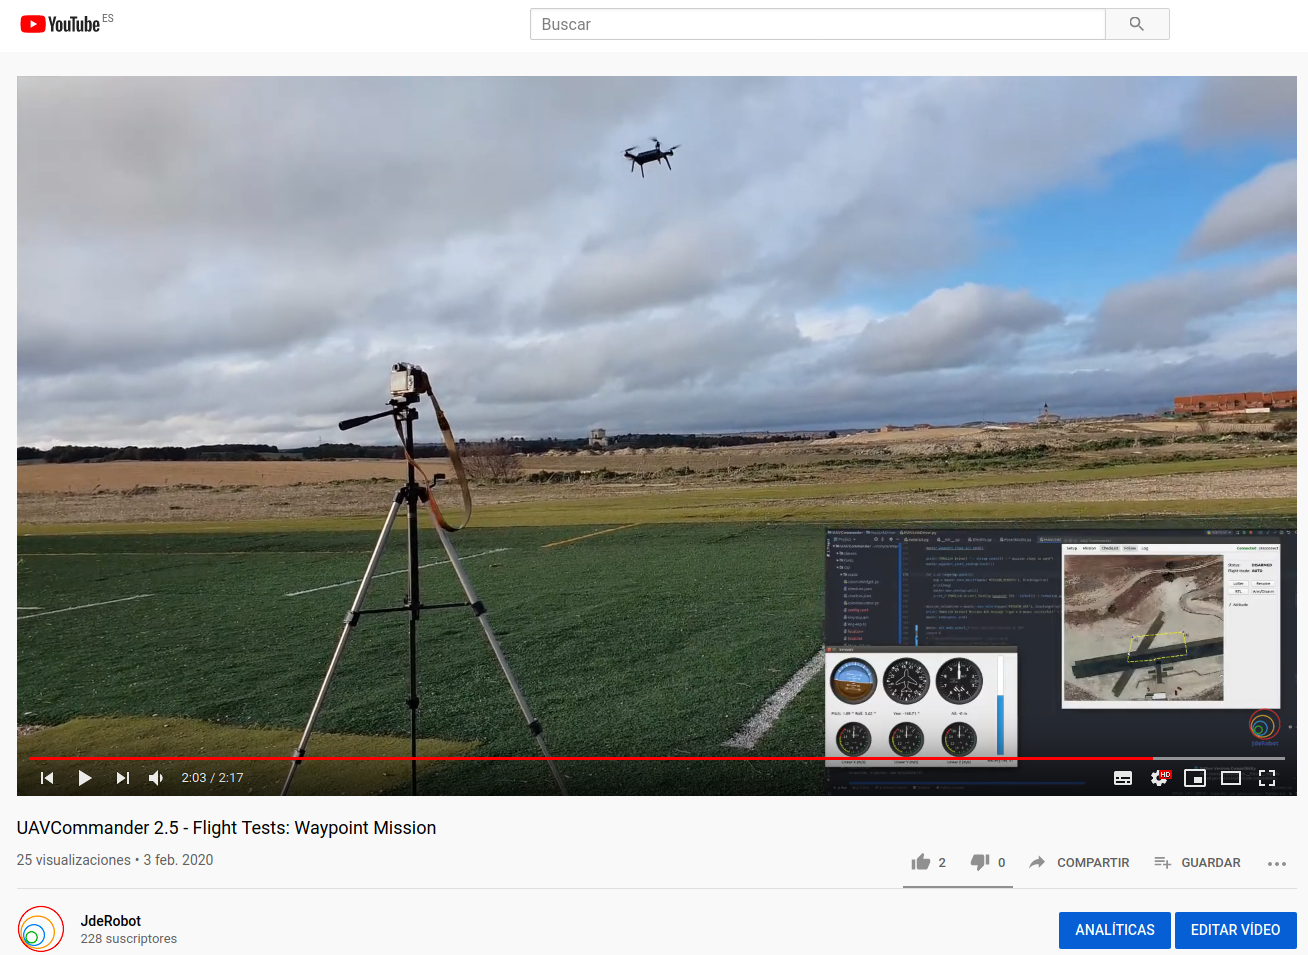
\includegraphics[height=6cm, width=0.9\linewidth]{prueba-pol-4.png}
        \caption{Aterrizaje y fin de la misión.}
        \label{fig:prueba-pol4}
    \end{subfigure}
     
    \caption{Vídeo con la prueba de vuelo para misiones polilínea.}
    \label{fig:prueba-pol}
\end{figure}

Tras realizar esta prueba integral se concluye que la aeronave completa satisfactoriamente la misión polilínea. El drone despega, recorre la secuencia de puntos de paso y aterriza en los puntos de paso especificados por el usuario a través de la aplicación desarrollada. Además, la posición de la aeronave se puede seguir en todo momento a través de la estación de tierra. Lo mismo sucede con otros parámetros de navegación como las velocidades o la actitud de la aeronave.

\section{Misión de patrón en simulación.}
Este experimento realiza en un entorno de simulación la creación de una misión por patrón, el envío a la aeronave y el seguimiento de la misión. La simulación permite la detección de errores sin poner en riesgo a la aeronave. La Figura \ref{fig:sim-patron} contiene unas capturas de pantalla realizadas durante la simulación. La secuencia de ejecución seguida ha sido:

\begin{enumerate}
    \item Lanzamiento de la simulación mediante un SITL de PX4 con Gazebo9. Ejecución de la aplicación.
    \item Establecimiento de la conexión entre estación terrestre y aeronave (ver caso de uso \ref{subsection:results-caso4}).
    \item Caracterización de la aeronave y carga de pago (ver caso de uso \ref{subsection:results-caso1}).
    \item Carga de una misión por patrón previamente confeccionada (ver caso de uso \ref{subsection:results-caso5} y Fig. \ref{fig:sim-patron1}).
    \item Validación de la misión creada.
    \item Comprobaciones pre-vuelo y envío de la misión a la aeronave.
    \item Inicio de la misión y seguimiento de la misma (ver caso de uso \ref{subsection:results-caso6} y Fig. \ref{fig:sim-patron2}).
    \item Aterrizaje y fin de la misión.
\end{enumerate}

\begin{figure}[h]
    \begin{subfigure}{0.5\textwidth}
        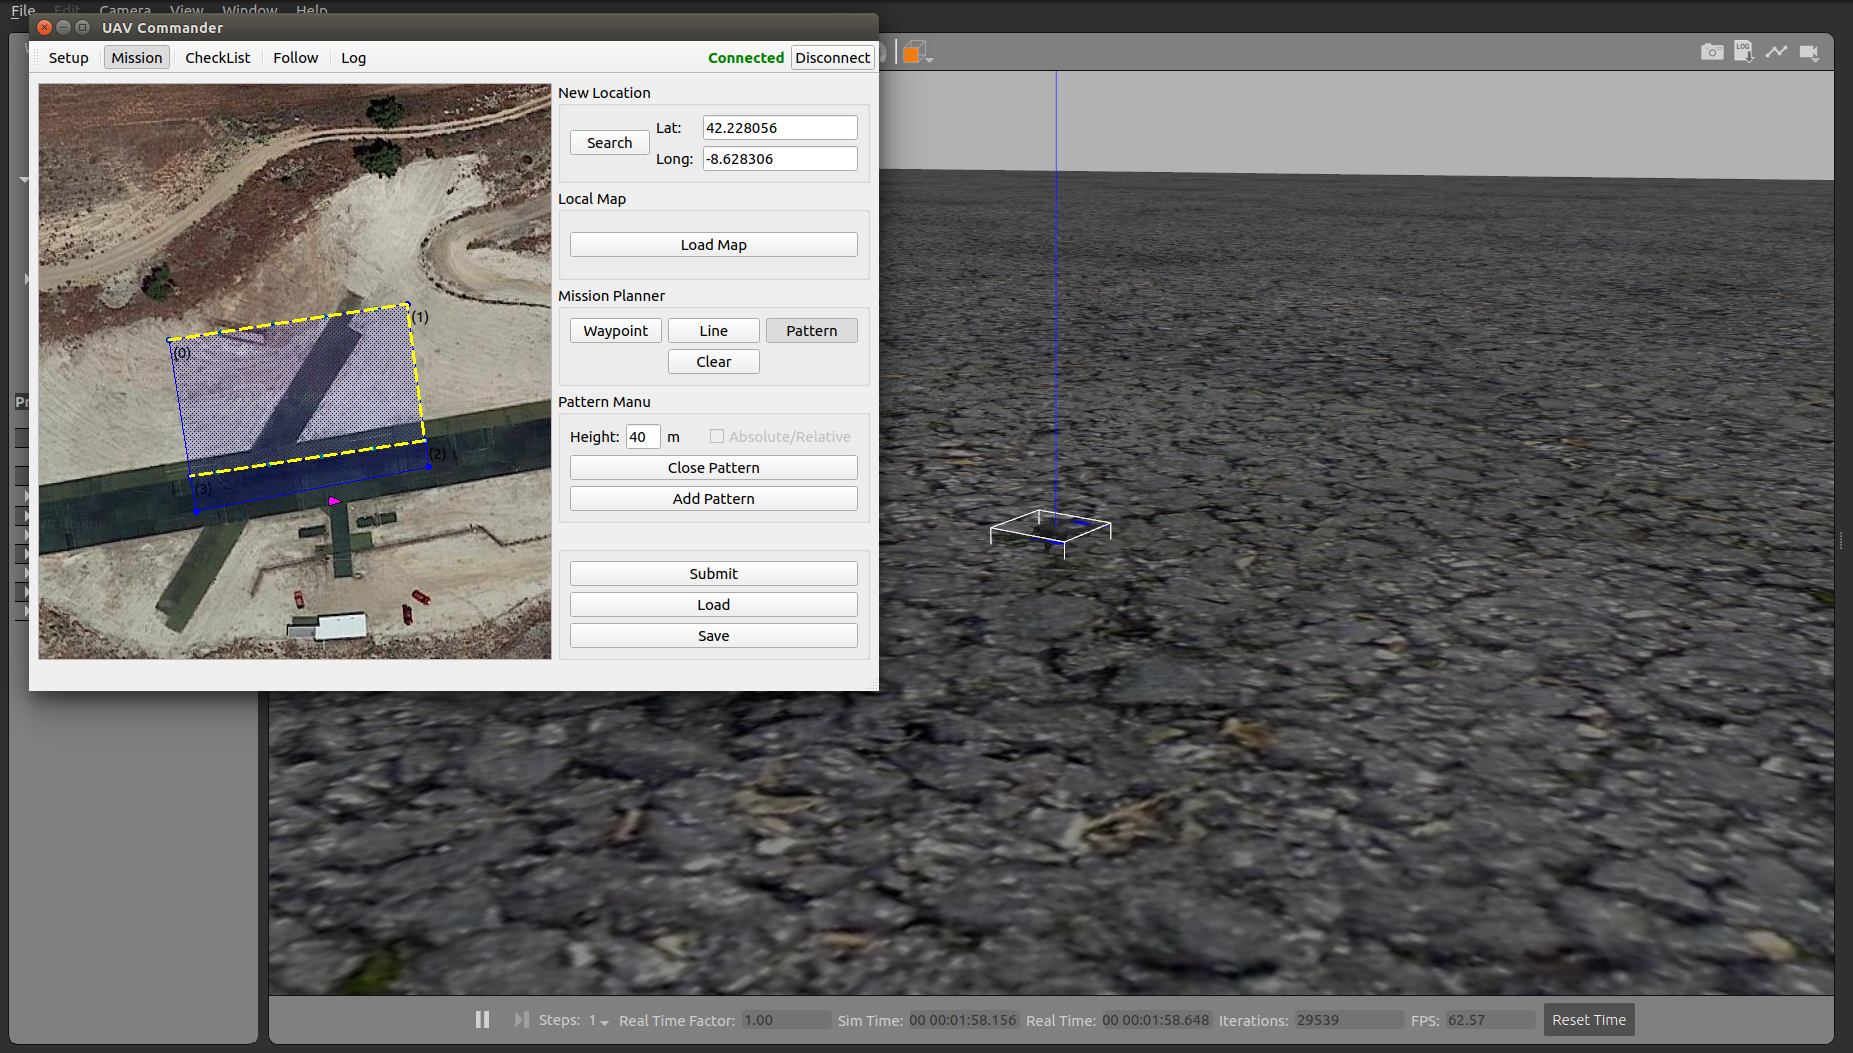
\includegraphics[width=0.9\linewidth]{sim-patron-1.png}
        \caption{Simulación de la creación de la misión.}
        \label{fig:sim-patron1}
    \end{subfigure}
    \begin{subfigure}{0.5\textwidth}
        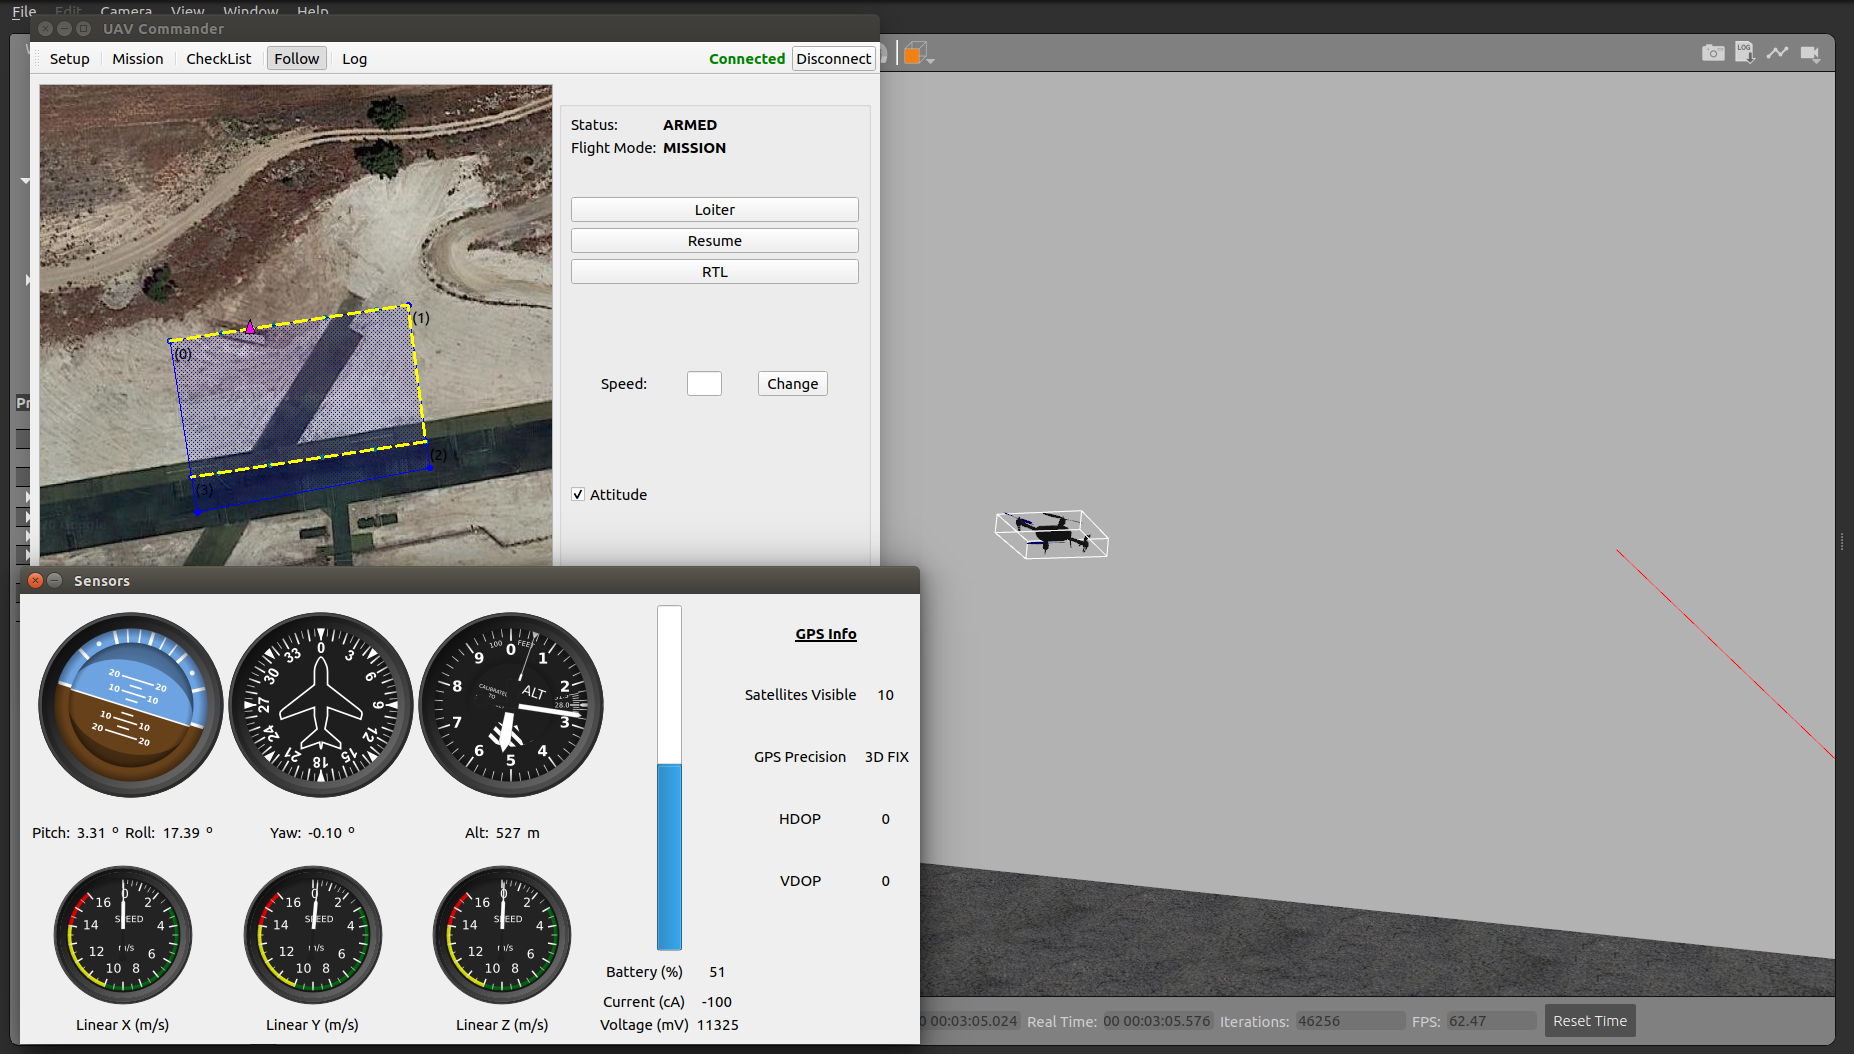
\includegraphics[width=0.9\linewidth]{sim-patron-2.png}
        \caption{Simulación del seguimiento de la misión.}
        \label{fig:sim-patron2}
    \end{subfigure}

    \caption{Simulación de vuelo para misiones por patrón.}
    \label{fig:sim-patron}
\end{figure}

Tras realizar la prueba en simulación y comprobar el buen funcionamiento de la aplicación se considera que el software ya está listo para realizar pruebas en real. Esta prueba en real se muestra en la siguiente sección.

\section{Prueba de vuelo para misiones por patrón.}
Este ensayo de vuelo reproduce una situación en la cual un operario carga una misión por patrón previamente creada, la envía a la aeronave y realiza el seguimiento de la misma. Se adjunta un enlace de un vídeo \footnote{https://youtu.be/tpmpdkG0CjM} con el experimento real. Además, la Figura \ref{fig:prueba-pol} muestra un fotograma del vídeo adjunto. \\

La secuencia de ejecución seguida durante la prueba de vuelo ha sido la siguiente:

\begin{enumerate}
    \item Ejecución de la aplicación y encendido del 3DR Solo junto a su emisora.
    \item Establecimiento de conexión entre ambos cuando el 3DR Solo ha establecido señal GPS (ver caso de uso \ref{subsection:results-caso4}).
    \item Caracterización de la aeronave y carga de pago (ver caso de uso \ref{subsection:results-caso1}).
    \item Carga de una misión por patrón previamente confeccionada (ver caso de uso \ref{subsection:results-caso5}).
    \item Validación de la misión creada.
    \item Comprobaciones pre-vuelo y envío de la misión a la aeronave.
    \item Inicio de la misión y seguimiento de la misma (ver caso de uso \ref{subsection:results-caso6}).
    \item Aterrizaje y fin de la misión.
\end{enumerate}

% Es importante destacar que algún aspecto menor del vídeo puede diferir con la versión actual, pues en el momento de grabación la aplicación se encontraba todavía en proceso de desarrollo.

%\begin{figure}[h]
%    \centering
%    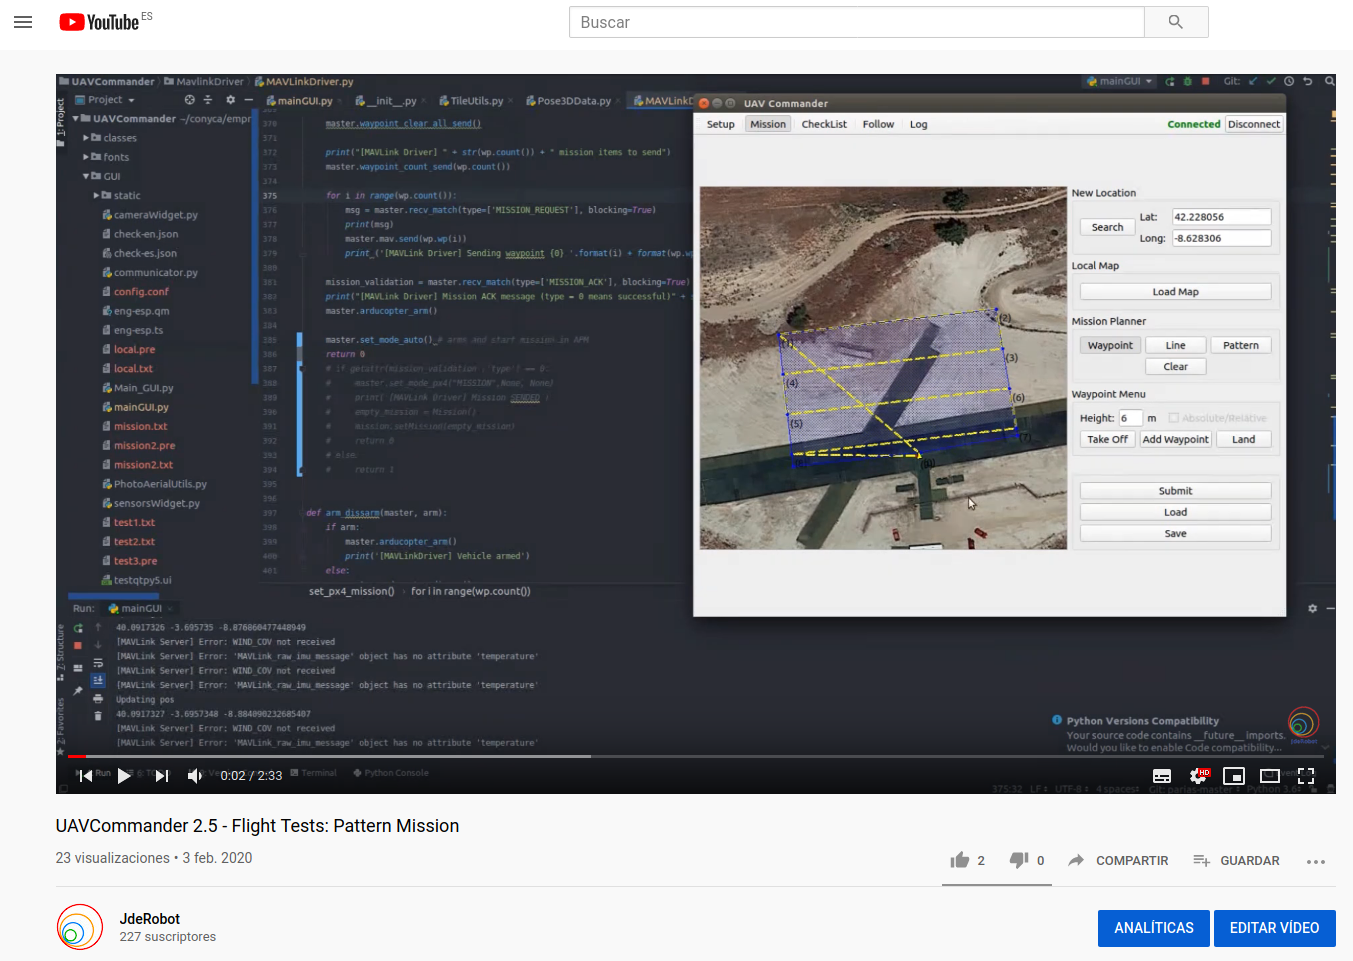
\includegraphics[width=0.9\textwidth]{prueba-patron.png}
%    \caption{Vídeo con la prueba de vuelo para misiones por patrón.}
%    \label{fig:prueba-patron}
%\end{figure}

\begin{figure}[h]
    \begin{subfigure}{0.5\textwidth}
        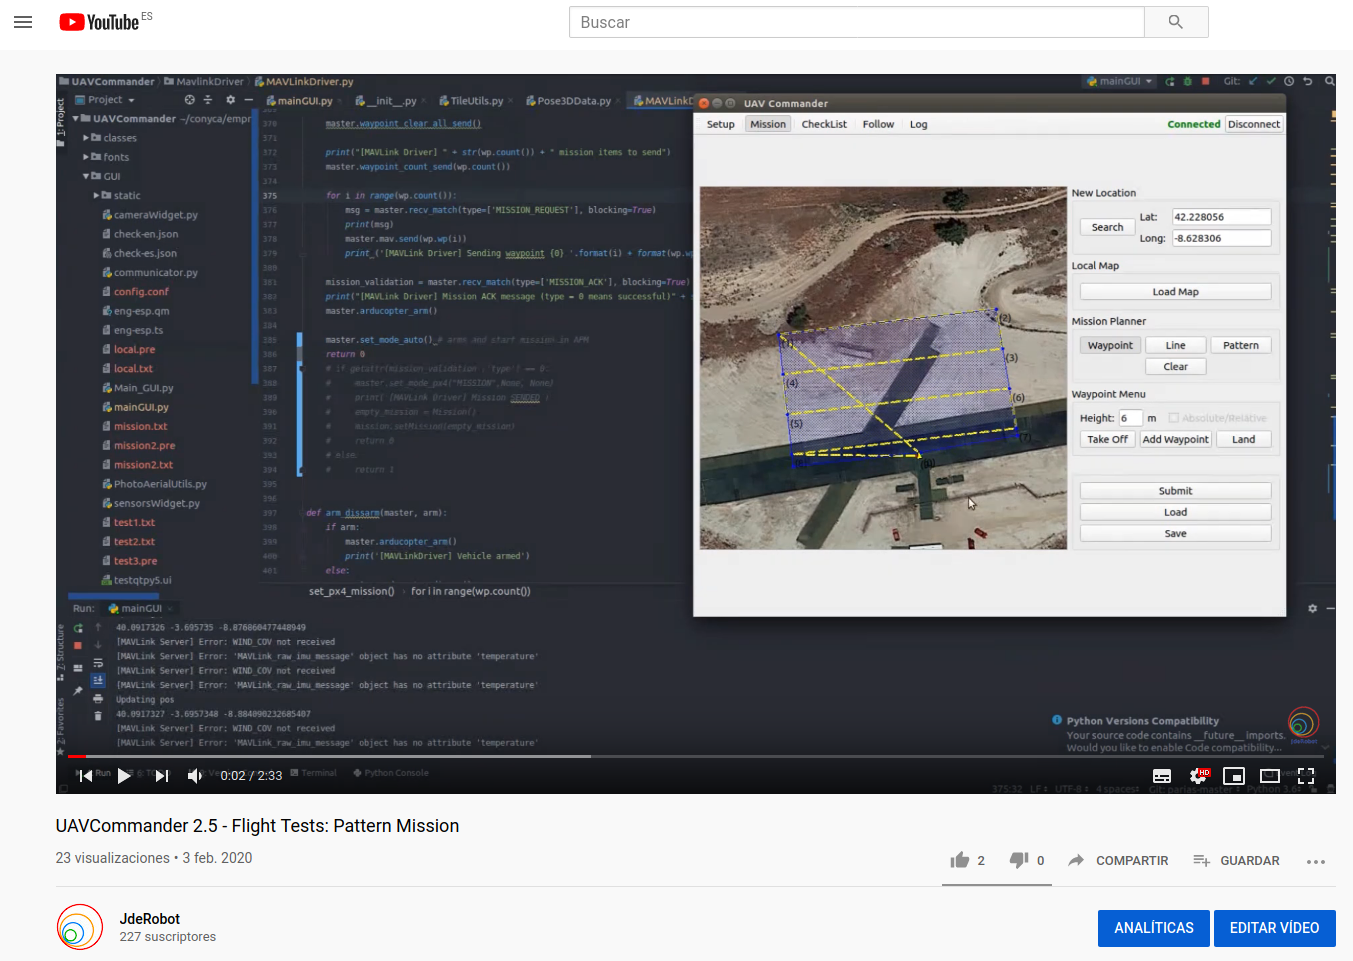
\includegraphics[height=6cm, width=0.9\linewidth]{prueba-patron.png}
        \caption{Creación de la misión por patrón.}
        \label{fig:prueba-patron1}
    \end{subfigure}
    \begin{subfigure}{0.5\textwidth}
        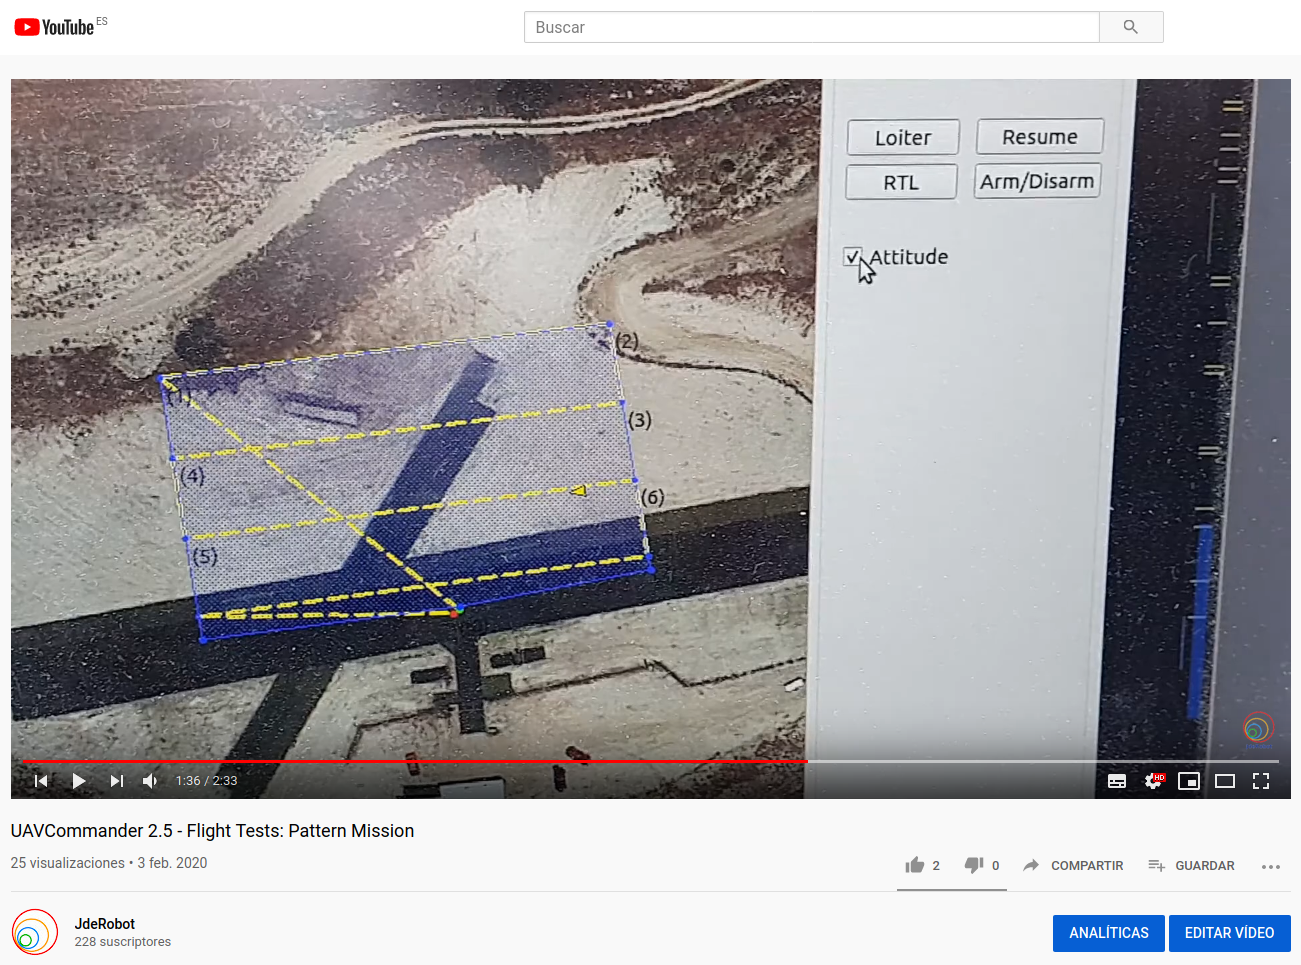
\includegraphics[height=6cm, width=0.9\linewidth]{prueba-patron-1.png}
        \caption{Seguimiento de la misión.}
        \label{fig:prueba-patron2}
    \end{subfigure}

    \caption{Vídeo con la prueba de vuelo para misiones por patrón.}
    \label{fig:prueba-patron}
\end{figure}

Tras realizar esta prueba integral se concluye que la aeronave completa satisfactoriamente la misión por patrón. La ruta se genera automáticamente tras seleccionar la región de escaneo. El drone recorre dicha ruta según la forma indicada. Además, la posición de la aeronave se puede seguir en todo momento a través de la estación de tierra. Lo mismo sucede con otros parámetros de navegación como las velocidades o la actitud de la aeronave.